\documentclass[a4paper,10pt]{article}
\usepackage{ctex}
\usepackage[utf8]{inputenc}
\usepackage{fancyhdr}
\usepackage{mflogo,texnames}
\usepackage{graphicx}
\usepackage{amssymb}
\usepackage{epstopdf}
\usepackage{listings}
\usepackage{color}
\definecolor{keywordcolor}{rgb}{0.8,0.1,0.5}
\definecolor{webgreen}{rgb}{0,.5,0}

\pagestyle{fancy}
\lhead{学号:1401214342}
\chead{姓名: 韩喆}
\rhead{}
\lfoot{Han Zhe(icst@pku)}
\cfoot{iampkuhz@gmail.com}
\rfoot{\thepage}

% word page layout
%\usepackage[top=2.54cm, bottom=2.54cm, left=3.18cm, right=3.18cm]{geometry}
\title{My First \LaTeX{} article}
\begin{document}
\begin{center}
\LARGE 算法课第 1次作业
\end{center}
\section{题目1 转换器}
  \normalsize
  \paragraph{问题转换}
  把原题对应到稳定婚姻问题:n条输出为n个女生,n条输入为n个男生。对于每个男生i,如果他和女生j在“输入i”的从源头开始的第k1个链接点交汇,表示女生j 是男生i排名第k1的心仪对象;反之,对每个女生j,如果她和男生i在“输出j” 的从末尾反向开始的第k2个连接点交汇,表示男生i是女生j排名第k2的心仪对象。原问题转换为给定了n 对男生和女生每个人对异性的喜好排序,求配对方式,使得配对稳定。
  \paragraph{证明存在性}
  对于转换后的问题求解:每个循环内,所有未配对的男生向未配对的女生中自己最喜欢的求婚,所有接到求婚的女生在向自己求婚的男生中选择自己最喜欢的结成一队。由稳定婚姻可以必然存在一个可行解,下面证明该解同样满足原来的限制条件。\
  反证,假设不存在,不放设输入i和输出j被配对(配对点在i的ip1位置,j的jp1 位置),但是存在:\
  (1)输入i上ip2位置(ip2<ip1),使得ip2在另一输出k上,且在k上ip2点之前k 已经接通
  (2)输出j上jp2位置下游存在一个输入电流i0的交点ip0
  由对称性,只考虑第(2)种情况。由i0 经过j,说明i0最后配对的对象在i0心中排名低于j,说明i0一定在之前的某轮向j表白且被拒了。j 没有选i0,说明j 选了比i0更好的(在j心中),但是实际j选的i没有i0 排名高,矛盾!所以按照上述方法求得的配对满足上下游限制要求,也就是可行解。
  \paragraph{求解算法}
  见“问题转换”\

\section{题目2 求最大n}
  \paragraph{$(a) n^2 $}
  由$n^2 \leqslant 10^{10} \times 60 \times 60$ \\ 得到 $n\leqslant6\times10^6$,所以n最大为$6\times10^6$
  \paragraph{$(b) n^3 $}
  由 $n^3\leqslant10^{10}\times60\times60$ \\ 得到 $n\leqslant33015 $,所以n最大为$33015$
  \paragraph{$(c) n^3 $}
  由 $100\times n^2\leqslant10^{10}\times60\times60$ \\ 得到 $n\leqslant6\times10^6$,所以n最大为$6\times10^5$
  \paragraph{$(d) n\log n$}
  令 $t=\log n$ $n\log n>n$得到$2^t\times t\leqslant10^{10}\times60\times60$,两边取log得到$t+\log t \leqslant 2\log6+12\log10$在区间$[0, 2\log6+12\log10]$ 二分查找,当区间长度小于0.000001 的时候停止得到$n\approx 2^{41.31191}$

\lstinputlisting[language=Java]{test.java}

  \paragraph{$(e) 2^n$}
  令$2^n \leqslant 10^{10} \times 60 \times 60$, 取$log$得到$n\leqslant 2\log6+12\log10$,n最大为$45$
  \paragraph{$(f) 2^{2^n}$}
  令$2^{2^n} \leqslant 10^{10} \times 60 \times 60$, 取$log$后再取$log$得到$n\leqslant \log{2\log6+12\log10}$,n最大为$5$

\section{题目3 比较大小}
  \subparagraph{如无特殊说明,本题证明中的$a<b$均表示 $$\lim_{n \to \infty}\frac{a}{b} = \infty$$}
  \paragraph{}
  由$$\log n<\sqrt n<n<n^2<2^n$$ 得到
  $$\sqrt{\log n}<\log n<\log n+3\times \log{\log n}<\log n+\frac{1}{3}\log n$$
  $$<(\log n)\times(\log n)<(\sqrt n)\times(\sqrt n)=n<n^2<2^n$$
  将上式每一个做2的指数,得到
  $$g_1=2^{\sqrt{\log n}}<2^{\log n}=n<2^{\log n+3\times \log{\log n}}=g_4$$
  $$<2^{\log n+\frac{1}{3}\log n}=g_3<2^{(\log n)\times(\log n)}=g_5$$
  $$<2^{(\sqrt n)\times(\sqrt n)}=2^n<2^{n^2}=g_7<2^{2^n}=g_6$$
\section{题目4 判断函数复杂度真假}
  \paragraph{(a)}
  false\\
  e.g.
  $$f(n)=1, g(n)=2$$
  then
  $$\log_2 f(n)=0, \log_2 g(n)=1$$
  thus
  $$O(\log_2 f(n))=O(0)\neq O(\log_2 g(n))=O(1)$$

  \paragraph{(b)}
  false\\
  e.g.
  $$f(n)=n+\log n, g(n)=n$$
  then
  $$O(f(n))=O(n)=O(g(n)), \log_2 f(n)=0, \log_2 g(n)=1$$
  thus
  $$O(2^{f(n)})=O(n\times 2^n)\neq O(2^{g(n)})=O(2^n)$$

  \paragraph{(c)}
  true\\
  given $f(n)\leqslant cg(n)$ for all $n\geqslant n_0$\\
  we have\\
  $(f(n))^2\leqslant c^2(g(n))^2$ for all $n\geqslant n_0$

\section{题目5 找到最短路径数目}
\paragraph{(算法思路)}
采用BFS,由近及远找到离起始点v的点。从开始点v作为结果集$R_0()$ 表示从v 一步走到的点数目(存储点集及其路径数),这里路径数为1。 之后第i 轮开始时从$R_{i-1}()$ 集合取出所有点,找到与他们直接链接的所有点,将其中未在之前判断过的点集中的点加入$R_i()$,其在$R_i()$中的路径数为所有通向它的$R_{i-1}()$集合中的点的路径数之和。等到搜索到目标点w停止,每个点至多扫描一次,每条边至多扫描一次,复杂度为$O(m+n)$

\paragraph{(代码)}
\begin{figure}[h]
2 \centering
3 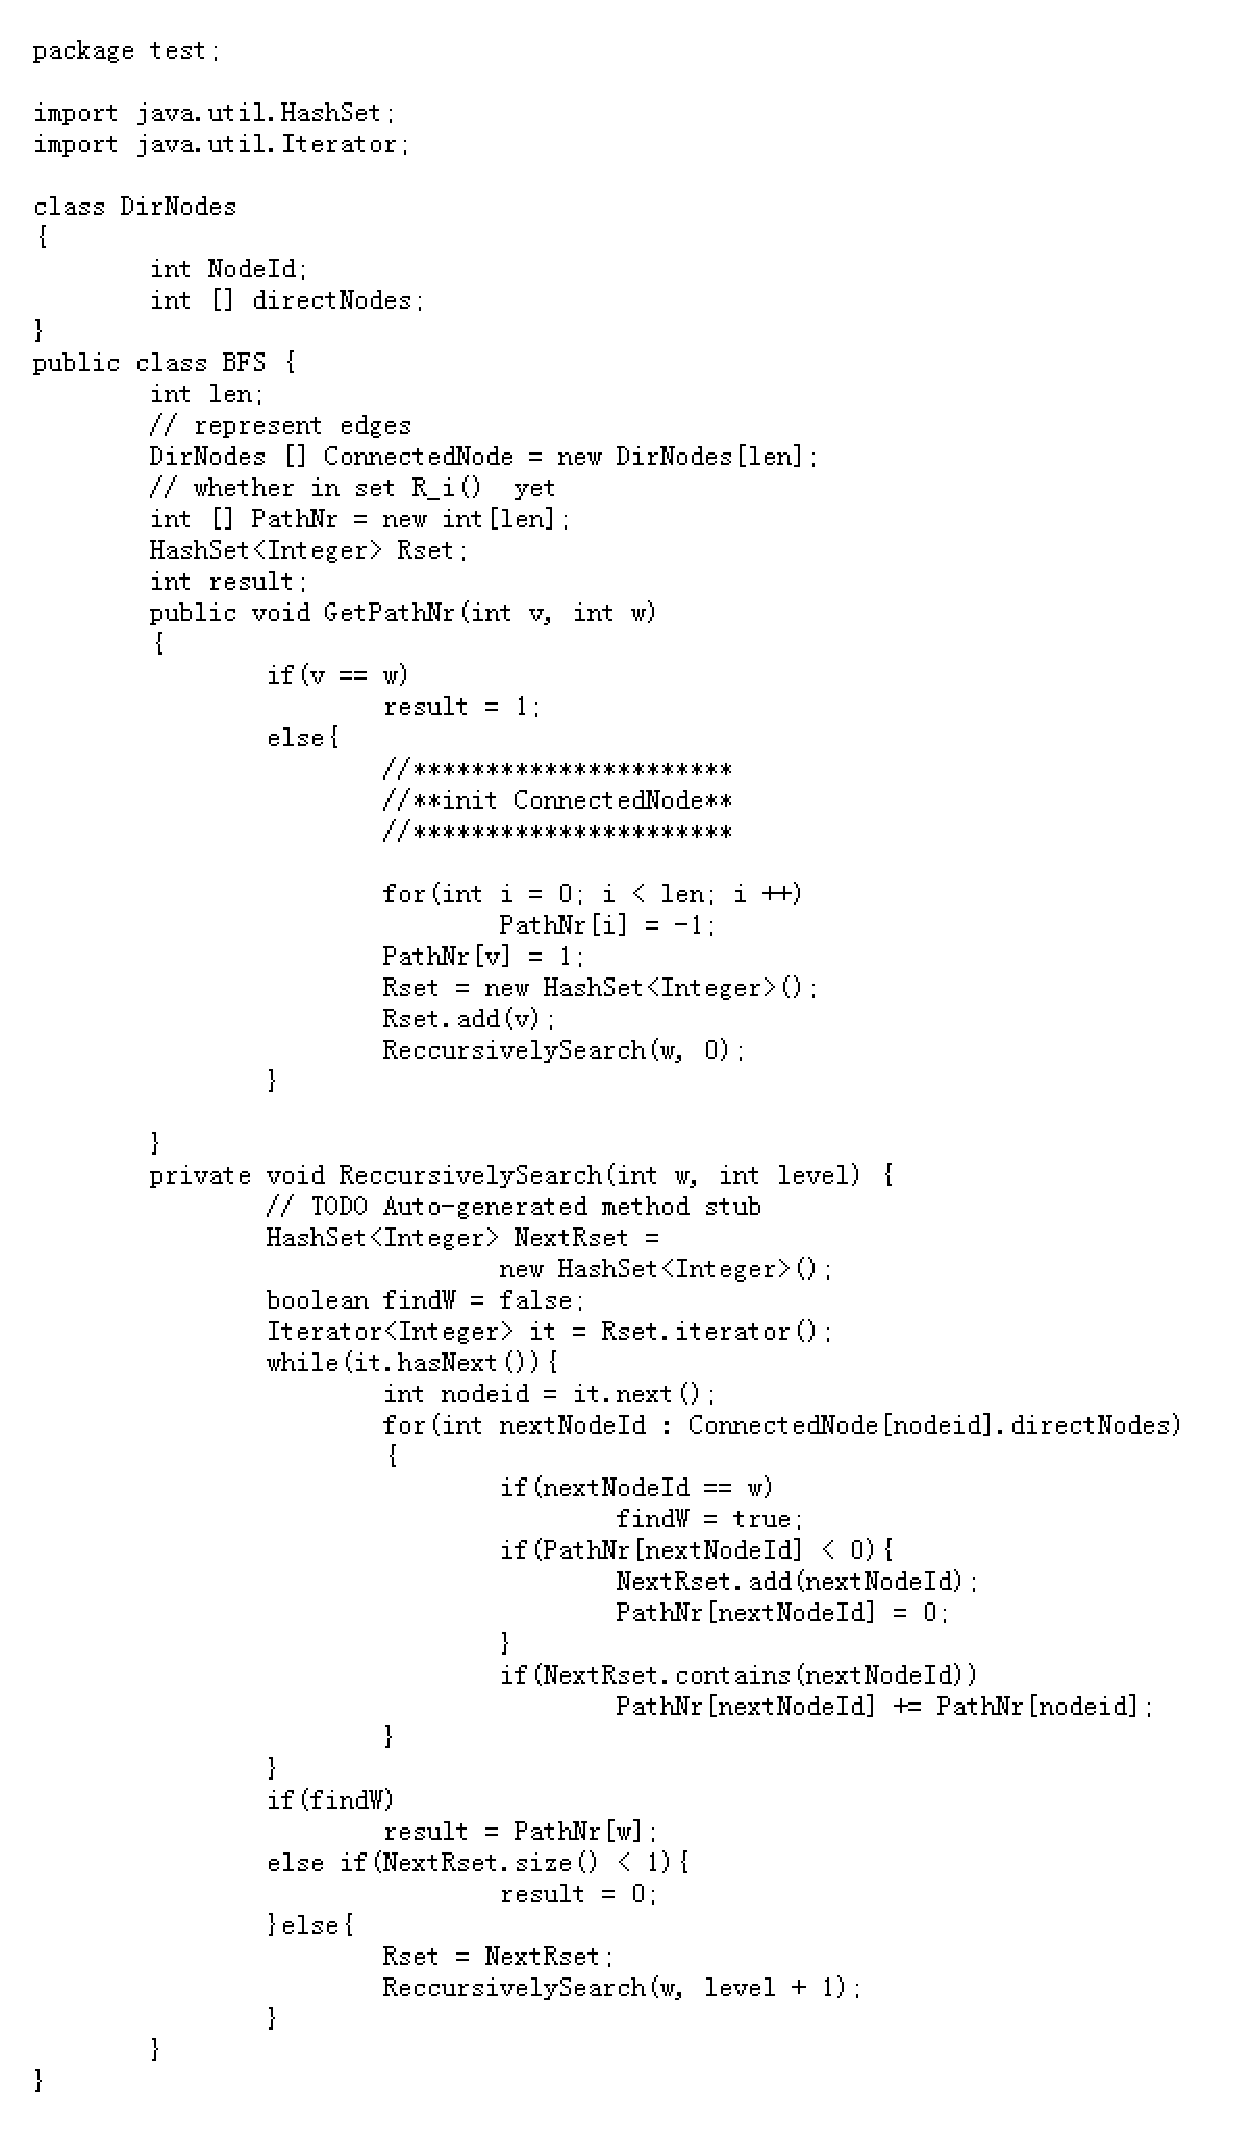
\includegraphics[width=0.8\textwidth]{1}
4 \end{figure}

\end{document}
